\documentclass[a4paper, 10pt, twocolumn]{article}
\usepackage[utf8]{inputenc}
\usepackage[T1]{fontenc}
\usepackage{graphicx}
\usepackage{lipsum}
\usepackage{geometry}
\usepackage{titlesec}
\usepackage{times}
\usepackage{hyperref}
\usepackage{amsmath}
\usepackage[linesnumbered,ruled,vlined]{algorithm2e}
\usepackage{listings}
\usepackage{color}
\geometry{a4paper, margin=0.75in}
%\geometry{left=2.5cm, right=2.5cm, top=2.5cm, bottom=2.5cm}
\definecolor{codegreen}{rgb}{0,0.6,0}
\definecolor{codegray}{rgb}{0.5,0.5,0.5}
\definecolor{codepurple}{rgb}{0.58,0,0.82}
\definecolor{backcolour}{rgb}{0.95,0.95,0.92}

\lstdefinestyle{mystyle}{
    backgroundcolor=\color{backcolour},
    commentstyle=\color{codegreen},
    keywordstyle=\color{magenta},
    numberstyle=\tiny\color{codegray},
    stringstyle=\color{codepurple},
    basicstyle=\ttfamily\footnotesize,
    breakatwhitespace=false,
    breaklines=true,
    captionpos=b,
    keepspaces=true,
    numbers=left,
    numbersep=5pt,
    showspaces=false,
    showstringspaces=false,
    showtabs=false,
    tabsize=2
}

\lstset{style=mystyle}
\begin{document}
\begin{titlepage}
    \centering
    \vspace{3.5cm}
    
\includegraphics[width=0.5\textwidth]{NU-logo.jpg}\par\vspace{1cm}
    
\includegraphics[width=0.5\textwidth]{FAST.png}\par\vspace{1cm}
    \vspace{1cm}
    {\scshape\LARGE\textbf {Codes for Applications of Graph Theory} \par}
    \vspace{1cm}
    {\scshape\LARGE\textbf {Fiber Optics Trajectory Optimiztion\\(Minimum Spanning Trees using Naive \& Efficient Prim's \& Kruskal's Algorithms)} \par}
    \vspace{1cm}
    {\scshape\Large Project Report \par}
    \vspace{1cm}
    {\scshape\Large Professor Dr. Nazish Kanwal (BCS-5E) \par}
    \vspace{1cm}
    {\scshape\Large Graph Theory (MT-3001) \par}
    \vspace{1cm}
    \begin{itemize}
    \item {\scshape\Large Muhammad Talha (K21-3349) \par}
    \vspace{0.25cm}
    \item {\scshape\Large Muhammad Hamza (K21-4579) \par}
    \vspace{0.25cm}
    \item {\scshape\Large Muhammad Salar (K21-4619) \par}
    \end{itemize}
    \vfill
    \vspace{1cm}    
    {Foundation of Advancement of Science and Technology \par}
    {National University of Computer and Emerging Sciences \par}
    {Department of Computer Science \par}
    {Karachi, Pakistan \par}
    {Thursday, November 31, 2023 \par}
\end{titlepage}

\begin{titlepage}
\onecolumn
\begin{abstract}
% Your abstract content here
This project aims to implement and compare different algorithms for finding minimum spanning trees (MSTs) in graphs, which are useful for solving various optimization problems. We use Python to code the naive and efficient versions of Prim’s and Kruskal’s algorithms and test them on randomly generated graphs with different sizes and densities. We measure the running time and memory usage of each algorithm and analyze the trade-offs between them. We also discuss some applications and limitations of MSTs in real-world scenarios.
\end{abstract}
\tableofcontents
\end{titlepage}

\twocolumn
\section{Introduction}
% Your introduction content here
Graph theory is a branch of mathematics that studies the properties and structures of graphs, which are abstract representations of objects and their pairwise relations. A graph consists of a set of vertices (or nodes) and a set of edges (or links) that connect some pairs of vertices. An edge can have a weight, which is a numerical value that indicates the cost or distance of the connection. A graph can be undirected, meaning that the edges are bidirectional, or directed, meaning that the edges have a direction from one vertex to another.

\subsection{Background}
One of the fundamental problems in graph theory is finding a spanning tree of a graph, which is a subgraph that contains all the vertices and is a tree, meaning that it has no cycles. A spanning tree can be used to connect all the vertices in a graph with the minimum number of edges, which is useful for network design, routing, clustering, and other applications. Among all the possible spanning trees of a graph, a minimum spanning tree (MST) is the one that has the minimum total weight of its edges. Finding an MST of a graph can help to minimize the cost or distance of the connections, which is desirable for many optimization problems.

There are several algorithms for finding an MST of a graph, each with different time and space complexities, and different advantages and disadvantages. In this project, we focus on two of the most well-known and widely used algorithms: Prim’s and Kruskal’s algorithms. Both algorithms are greedy, meaning that they make the locally optimal choice at each step, and both algorithms can handle undirected graphs with positive edge weights. However, they differ in the way they construct the MST and the data structures they use.

\subsection{Problem Statement}
The project aims to explore efficient fiber optic trajectory management by comparing the efficiency of two different algorithms, namely naive and efficient versions of Prim's and Kruskal's algorithms, in finding minimum spanning trees. The focus is on understanding the complexities and trade-offs involved in each algorithm and their practical implications. Firstly, it ensures uninterrupted connectivity by minimizing disruptions and contributes to minimizing costs. By effectively allocating resources and utilizing MST algorithms, organizations can cater to growing bandwidth demands while maintaining optimal network speeds.

\section{Programming Design}
\subsection{Algorithm Description}
\subsubsection{Prim’s Algorithm}
Prim’s algorithm starts with an arbitrary vertex and grows the MST by adding the cheapest edge that connects a vertex in the MST to a vertex outside the MST until all the vertices are included. Prim’s algorithm can be implemented using a priority queue to store the vertices and their distances to the MST, and an array to store the parent of each vertex in the MST. The naive version of Prim’s algorithm uses a simple list as the priority queue, which has a linear time complexity for finding and removing the minimum element. The efficient version of Prim’s algorithm uses a binary heap as the priority queue, which has a logarithmic time complexity for finding and removing the minimum element, and for updating the distances of the vertices.
\subsubsection{Kruskal’s Algorithm}
Kruskal’s algorithm starts with an empty set of edges and adds the cheapest edge that does not create a cycle until the MST is formed. Kruskal’s algorithm can be implemented using a disjoint-set data structure to store the connected components of the graph, and a sorted list of edges by their weights. The naive version of Kruskal’s algorithm uses a simple list as the disjoint set and insertion sort, which has a quadratic time complexity for finding and merging the components. The efficient version of Kruskal’s algorithm uses a tree-based representation with path compression and union by rank as the disjoint set and merge sort, which has a logarithmic time complexity for finding and merging the components.

\onecolumn
\subsection{Implementation}
%\textbf{Naive:\\}
\begin{algorithm}
\caption{Naive Prim's Algorithm}
\KwData{Graph $G$}
\KwResult{Minimum Spanning Tree $MST$}
\BlankLine
$MST \leftarrow \{\}$\;
$start\_vertex \leftarrow G.\text{getAnyVertex}()$\;
\text{markAsVisited}($start\_vertex$)\;

\While{\text{not} allVerticesVisited()}{
    $min\_edge \leftarrow$ \text{findMinimumEdge}()\;
    $MST$.add($min\_edge$)\;
    \text{markAsVisited}($min\_edge.\text{endVertex}$)\;
}
\Return $MST$\;
\end{algorithm}
%\textbf{Efficient:\\}
\begin{algorithm}
\caption{Effiecient Prim's Algorithm with Min Heap}
\KwData{Graph $G$}
\KwResult{Minimum Spanning Tree $MST$}
\BlankLine
$MST \leftarrow \{\}$\;
$priority\_queue \leftarrow$ initializeMinHeap()\;
$start\_vertex \leftarrow G.\text{getAnyVertex}()$\;
\ForEach{vertex $v$ in $G.\text{vertices}$}{
    \If{$v$ is not $start\_vertex$}{
        $priority\_queue.\text{insert}(v, \infty)$\;
    }
}
\While{$\neg priority\_queue.\text{isEmpty}()$}{
    $current \leftarrow priority\_queue.\text{extractMin}()$\;

    \ForEach{neighbor $n$ of $current$}{
        \If{$n$ is in $priority\_queue$ \text{and} $G.\text{weight}(current, n) <$ priority\_queue.\text{getPriority}($n$)}{
            $priority\_queue.\text{decreasePriority}(n, G.\text{weight}(current, n))$\;
        }
    }
    $MST.\text{addEdge}(current, priority\_queue.\text{getPriority}(current))$\;
}
\Return $MST$\;
\end{algorithm}

%\textbf{Naive:\\}
\begin{algorithm}
\caption{Naive Kruskal's Algorithm with Insertion Sort}
\KwData{Graph $G$}
\KwResult{Minimum Spanning Tree $MST$}
\BlankLine
$MST \leftarrow \{\}$\;
$edges \leftarrow$ initializeList()\;
$disjoint\_set \leftarrow$ initializeDisjointSet($G.\text{vertices}$)\;
\ForEach{edge $e$ in $G.\text{edges}$}{
    $edges.\text{insert}(e)$\;
}
$edges.\text{insertionSort}()$\;
\ForEach{edge $e$ in $edges$}{
    \If{$\text{find}(e.\text{startVertex}, disjoint\_set.\text{parent}) \neq \text{find}(e.\text{endVertex}, disjoint\_set.\text{parent})$}{
        $MST.\text{addEdge}(e.\text{startVertex}, e.\text{endVertex})$\;
        $disjoint\_set.\text{union}(e.\text{startVertex}, e.\text{endVertex})$\;
    }
}
\Return $MST$\;
\end{algorithm}

%\textbf{Efficient:\\}
\begin{algorithm}
\caption{Efficient Kruskal's Algorithm with Merge Sort}
\KwData{Graph $G$}
\KwResult{Minimum Spanning Tree $MST$}
\BlankLine
$MST \leftarrow \{\}$\;
$edges \leftarrow$ initializeList($G.\text{edges}$)\;
$disjoint\_set \leftarrow$ initializeDisjointSet($G.\text{vertices}$)\;
$edges.\text{mergeSort}()$\;
\ForEach{edge $e$ in $edges$}{
    \If{$\text{find}(e.\text{startVertex}, disjoint\_set.\text{parent}) \neq \text{find}(e.\text{endVertex}, disjoint\_set.\text{parent})$}{
        $MST.\text{addEdge}(e.\text{startVertex}, e.\text{endVertex})$\;
        $disjoint\_set.\text{union}(e.\text{startVertex}, e.\text{endVertex})$\;
    }
}
\Return $MST$\;
\end{algorithm}

\twocolumn
\section{Experimental Setup}
In this section, we detail the experimental setup for testing and comparing the performance of Prim’s and Kruskal’s algorithms implemented in Python. Additionally, we introduce the experimental design for a secondary language, C++, to provide a basis for comparison.
\subsection{Python Implementation}
We use Python as the primary programming language for this project, and use the following modules and libraries:
\begin{itemize}
    \item random: to generate random numbers and graphs
    \item matplotlib: to plot the graphs and the results
    \item time: to measure the running time of the algorithms
\end{itemize}
We define functions to implement the naive and efficient versions of Prim’s and Kruskal’s algorithms. The functions take a graph as an input and return mst, cost and time, where mst is the MST of the graph as a list of edges, the cost is the total weight of the MST and time is the running time of the algorithm in seconds. The functions are:
\begin{itemize}
    \item primMST(graph, points, V): the naive version of Prim’s algorithm, which uses a list as the priority queue
    \item primMST(graph, points, V): the efficient version of Prim’s algorithm, which uses a binary heap as the priority queue
    \item kruskalMST(graph, points, V): the naive version of Kruskal’s algorithm, which uses a list as the disjoint-set and insertion sort
    \item kruskalMST(graph, points, V): the efficient version of Kruskal’s algorithm, which uses a tree-based representation with path compression and union by rank as the disjoint-set and merge sort
\end{itemize}
We also define a function to generate a random graph with a given number of vertices and random density, which is the ratio of the number of edges to the maximum possible number of edges. The function is:
\begin{itemize}
    \item generateRandomGraph(N): a function that creates a new graph with n vertices and m edges, where m is the closest integer to density * n * (n - 1) / 2, and the edge weights are randomly chosen
\end{itemize}
We use the following experimental setup to test and compare the performance of the algorithms:
\begin{itemize}
    \item We generate random graphs for each combination of n = 10, 100, 1000, 10000.
    \item We run each algorithm on each graph and record the output and the performance metrics.
    \item We also plot some examples of graphs and their MSTs, and discuss the differences between the algorithms.
    \item We discuss the differences between the algorithms and their respective performance.
\end{itemize}
\subsection{C++ Implementation}
To provide a basis for comparison, we replicate the experimental setup in C++ using similar implementations for Prim’s and Kruskal’s algorithms. We follow the same steps and record performance metrics for C++. This allows us to analyze and compare the efficiency of the algorithms in both Python and C++.

\onecolumn
\subsection{Code Snippets(Python)}
\subsubsection{General Code}
\begin{lstlisting}[language=Python, caption={Python code to generate a random graph}]
import random

def generateRandomGraph(N):
    # Initialize an empty list of points
    points = []

    # Loop through N times
    for _ in range(N):
        # Generate a random point with x and y coordinates between 0 and 100
        x = random.randint(0, 100)
        y = random.randint(0, 100)
        # Append the point to the list
        points.append((x, y))

    # Initialize an empty adjacency matrix with weights
    graph = [[0 for _ in range(N)] for _ in range(N)]

    # Loop through all vertices to determine random degrees
    for i in range(N):
        # Generate a random degree for the current vertex
        degree = random.randint(1, N - 1)  
        # Ensure that degree is at least 1 and at most N-1

        # Create a list of potential neighbors (excluding self)
        potential_neighbors = [j for j in range(N) if j != i]

        # Randomly choose 'degree' neighbors for the current vertex
        neighbors = random.sample(potential_neighbors, degree)

        # Update the adjacency matrix with random weights for the chosen edges
        for neighbor in neighbors:
            weight = random.randint(1, 10)
            graph[i][neighbor] = weight
            graph[neighbor][i] = weight  # Assuming the graph is undirected

    # Return the graph, the points, and the number of vertices
    return graph, points, N
\end{lstlisting}
\begin{lstlisting}[language=Python, caption={Python code to find parent}]
def find(parent, i):
    # If the current element is its own parent, it is the root of the set
    if parent[i] == i:
        return i
    # Recursively find the root of the set to which 'i' belongs
    return find(parent, parent[i])
\end{lstlisting}
\begin{lstlisting}[language=Python, caption={Python code to perform the union of two sets represented by their set representatives}]
def union(parent, rank, x, y):
    # Find the set representatives (roots) of the sets to which 'x' and 'y' belong
    xroot = find(parent, x)
    yroot = find(parent, y)

    # Compare the ranks of the sets to determine which one to make the parent
    if rank[xroot] < rank[yroot]:
        parent[xroot] = yroot  # Attach the set with lower rank to the one 
        #with higher rank
    elif rank[xroot] > rank[yroot]:
        parent[yroot] = xroot  # Attach the set with lower rank to the one with 
        #higher rank
    else:
        parent[yroot] = xroot  # Attach 'yroot' to 'xroot' arbitrarily
        rank[xroot] += 1  # Increment the rank of the set with the new parent
\end{lstlisting}
\newpage
\begin{lstlisting}[language=Python, caption={Python code to display graph and MST}]

def plotGraph(graph, points, parent, V, animated=False):
    fig, (ax1, ax2) = plt.subplots(1, 2, figsize=(10, 5))
    ax1.set_title("Original Graph")
    ax2.set_title("Minimum Spanning Tree")

    # Scatter points on both subplots
    for i in range(V):
        ax1.scatter(points[i][0], points[i][1], color="red")
        ax2.scatter(points[i][0], points[i][1], color="green")

    # Plot all edges in the original graph
    for i in range(V):
        for j in range(i + 1, V):
            if graph[i][j] > 0:
                ax1.plot([points[i][0], points[j][0]], [points[i][1], points[j][1]], 
                color="black")
                ax1.text((points[i][0] + points[j][0]) / 2, 
                (points[i][1] + points[j][1]) / 2,
                         str(graph[i][j]), color="black")

    if animated:
        line, = ax2.plot([], [], color="blue")
        text = ax2.text(0, 0, "", color="blue")

        def update(frame):
            i, j = frame
            x = [points[i][0], points[j][0]]
            y = [points[i][1], points[j][1]]
            line.set_data(x, y)
            text.set_position(((x[0] + x[1]) / 2, (y[0] + y[1]) / 2))
            text.set_text(str(graph[i][j]))

        ani = FuncAnimation(fig, update, frames=[(parent[i], i) for i in range(1, V)], 
        interval=2500, repeat=False)
        plt.close()  # To prevent the plot from showing up inline
        return ani
    else:
        # Plot edges in the minimum spanning tree
        for i in range(1, V):
            j = parent[i]
            ax2.plot([points[i][0], points[j][0]], [points[i][1], points[j][1]], 
            color="blue")
            ax2.text((points[i][0] + points[j][0]) / 2, (points[i][1] + points[j][1]) / 2,
                     str(graph[i][j]), color="blue")

        plt.show()
\end{lstlisting}
\newpage
\subsubsection{Prim's Code}
\begin{lstlisting}[language=Python, caption={Python code to find minimum key}]
def minKey(key, mstSet, V):
    # Initialize min value
    min_val = float('inf')
    min_index = -1

    # Loop through all the vertices
    for v in range(V):
        # If the vertex is not in the mstSet and has a smaller key value than 
        # the current min
        if mstSet[v] == False and key[v] < min_val:
            # Update the min value and index
            min_val = key[v]
            min_index = v

    # Return the index of the vertex with the minimum key value
    return min_index


\end{lstlisting}
\begin{lstlisting}[language=Python, caption={Python code for Naive Prim's}]
def primMST(graph, V):
    # Array to store constructed minimum spanning tree
    parent = [None] * V

    # Key values used to pick the minimum weight edge in the cut
    key = [float('inf')] * V

    # To represent the set of vertices not yet included in the minimum spanning tree
    mstSet = [False] * V

    # Always include the first vertex in the minimum spanning tree
    key[0] = 0  # Make key 0 so that this vertex is picked as the first vertex
    parent[0] = -1  # The first node is always the root of the minimum spanning tree

    # The minimum spanning tree will have V vertices
    for _ in range(V):
        # Pick the vertex with the minimum key value from the set of vertices not 
        #yet included in the minimum spanning tree
        u = minKey(key, mstSet, V)

        # Add the picked vertex to the mstSet
        mstSet[u] = True

        # Update the key value and parent index of the adjacent vertices of the picked 
        #vertex.
        # Consider only those vertices which are not yet included in the 
        #minimum spanning tree
        for v in range(V):
            # graph[u][v] is non-zero only for adjacent vertices of mstSet[u] is 
            #not in mstSet,
            # update the key only if graph[u][v] is smaller than key[v]
            if graph[u][v] > 0 and mstSet[v] == False and key[v] > graph[u][v]:
                key[v] = graph[u][v]
                parent[v] = u

    # Return the parent array
    return parent
\end{lstlisting}
\newpage
\begin{lstlisting}[language=Python, caption={Python code to find minimum key using Heap}]
def minKey(key, mstSet, V, heap):
    # This function extracts the vertex with the minimum key value from the heap
    # and ensures that the selected vertex has not been included in the MST yet.

    # Continue extracting elements from the heap until it is empty
    while heap:
        min_val, u = heapq.heappop(heap)  # Extract the minimum value and 
        # corresponding vertex from the heap

        # Check if the selected vertex 'u' has not been included in the MST yet
        if not mstSet[u]:
            return u  # Return the selected vertex with the minimum key value

    # If the heap is empty, return None (this should not happen in the context of 
    # Prim's algorithm)
    return None
\end{lstlisting}
\begin{lstlisting}[language=Python, caption={Python code for Efficient Prim's Algorithm}]
def primMST(graph, V):
    # Initialize arrays to store the parent of each vertex in the MST,
    # key values, MST set, and a heap for efficient key value extraction
    parent = [None] * V
    key = [(float('inf'), i) for i in range(V)]  # Initialize key values to infinity
    mstSet = [False] * V
    heap = [(0, 0)]  # Start with vertex 0 and key value 0 in the heap

    parent[0] = -1  # Vertex 0 is the starting point, and it has no parent
    key[0] = (0, 0)  # Key value for the starting vertex is set to 0

    # Iterate through all vertices to build the MST
    for _ in range(V):
        # Extract the vertex with the minimum key value from the heap
        u = minKey(key, mstSet, V, heap)
        mstSet[u] = True  # Add the selected vertex to the MST

        # Explore adjacent vertices and update key values and parents
        for v in range(V):
            # Check if there is an edge from u to v, v is not in MST, and
            # the weight of the edge is less than the current key value for v
            if graph[u][v] > 0 and not mstSet[v] and key[v][0] > graph[u][v]:
                key[v] = (graph[u][v], v)  # Update key value for v
                parent[v] = u  # Set u as the parent of v in the MST
                heapq.heappush(heap, key[v])  # Push the updated key to the heap

    # Return the array containing the parent of each vertex in the MST
    return parent
\end{lstlisting}
\newpage
\subsubsection{Kruskal's Code}
\begin{lstlisting}[language=Python, caption={Python code for Naive Kruskal Algorithm using Insertion Sort}]
def kruskalMST(graph, points, V):
    result = []  # Store the result MST
    i = 0  # An index variable for sorted edges
    e = 0  # An index variable for the result

    # Initialize parent and rank arrays
    parent = [i for i in range(V)]
    rank = [0] * V

    # Sort all the edges in non-decreasing order of their weight
    edges = []
    for u in range(V):
        for v in range(u + 1, V):
            if graph[u][v] != 0:
                edges.append((u, v, graph[u][v]))
    edges.sort(key=lambda x: x[2])

    while e < V - 1:
        u, v, w = edges[i]
        i += 1
        x = find(parent, u)
        y = find(parent, v)

        if x != y:
            e += 1
            result.append((u, v, w))
            union(parent, rank, x, y)

    return result
\end{lstlisting}
\begin{lstlisting}[language=Python, caption={Python code for Efficient Kruskal Algorithm using Merge Sort}]
def kruskalMST(graph, points, V):
    result = []  # Store the result MST
    i = 0  # An index variable for sorted edges
    e = 0  # An index variable for the result

    # Initialize parent and rank arrays
    parent = [i for i in range(V)]
    rank = [0] * V

    # Sort all the edges in non-decreasing order of their weight
    edges = []
    for u in range(V):
        for v in range(u + 1, V):
            if graph[u][v] != 0:
                edges.append((u, v, graph[u][v]))
    edges = sorted(edges, key=lambda x: x[2])  # Sort using the built-in sorted() function

    while e < V - 1:
        u, v, w = edges[i]
        i += 1
        x = find(parent, u)
        y = find(parent, v)

        if x != y:
            e += 1
            result.append((u, v, w))
            union(parent, rank, x, y)

    return result
    
\end{lstlisting}
\newpage
\subsubsection{Python Code Output for V = 10}
\begin{center}
    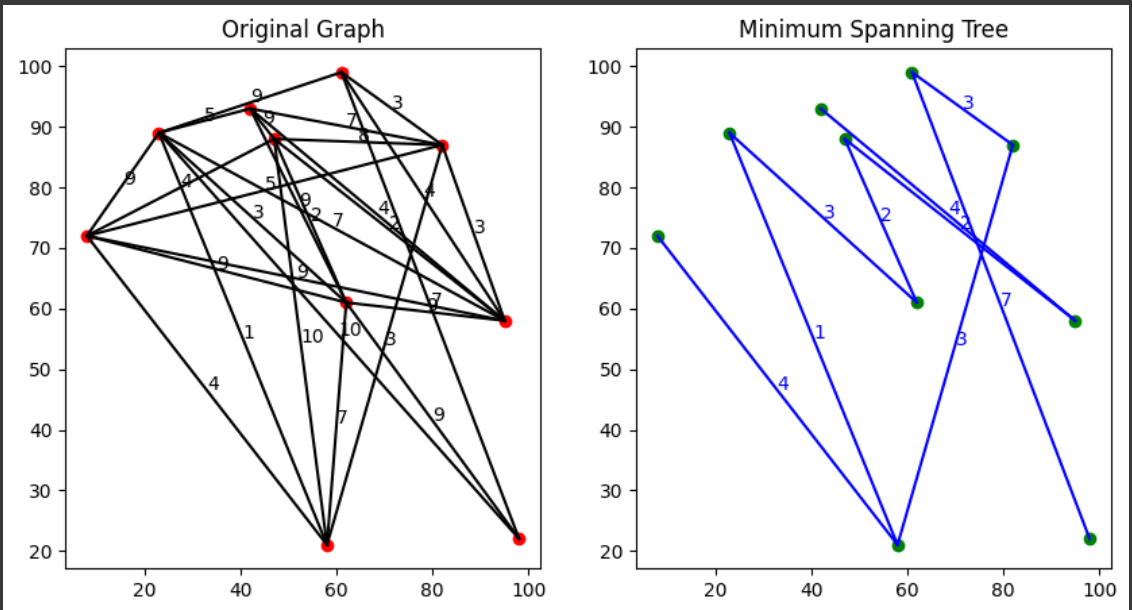
\includegraphics[width=0.75\textwidth]{kruskaleffecient.png}\par\vspace{1cm}
\end{center}

\subsection{Code Snippets(C++)}
\subsubsection{Prim's Code}
\begin{lstlisting}[language=C++, caption={C++ code for Naive Prim's  Algorithm}]
#include <limits.h>
#include <stdio.h>
#include <stdlib.h>
#include <time.h>
#include <sys/time.h> // for measuring execution time
#include <math.h>
#include <bits/stdc++.h>

using namespace std;

struct Point {
    int x, y;
};

struct AdjListNode {
    int dest;
    int weight;
    struct AdjListNode* next;
};

struct AdjList {
    struct AdjListNode* head;
};

struct Graph {
    int V;
    struct AdjList* array;
};

struct AdjListNode* newAdjListNode(int dest, int weight) {
    struct AdjListNode* newNode = (struct AdjListNode*)malloc(sizeof(struct AdjListNode));
    newNode->dest = dest;
    newNode->weight = weight;
    newNode->next = NULL;
    return newNode;
}

struct Graph* createGraph(int V) {
    struct Graph* graph = (struct Graph*)malloc(sizeof(struct Graph));
    graph->V = V;
    graph->array = (struct AdjList*)malloc(V * sizeof(struct AdjList));

    for (int i = 0; i < V; ++i)
        graph->array[i].head = NULL;

    return graph;
}

void addEdge(struct Graph* graph, int src, int dest, int weight) {
    struct AdjListNode* newNode = newAdjListNode(dest, weight);
    newNode->next = graph->array[src].head;
    graph->array[src].head = newNode;

    newNode = newAdjListNode(src, weight);
    newNode->next = graph->array[dest].head;
    graph->array[dest].head = newNode;
}

int calculateWeight(struct Point p1, struct Point p2) {
    // Calculate weight (distance) between two points (Euclidean distance)
    return (int)sqrt(pow(p1.x - p2.x, 2) + pow(p1.y - p2.y, 2));
}


void printGraph(struct Graph* graph) {
    int V = graph->V;
    printf("Randomly Generated Graph:\n");
    for (int i = 0; i < V; ++i) {
        struct AdjListNode* pCrawl = graph->array[i].head;
        printf("Vertex %d: ", i);
        while (pCrawl != NULL) {
            printf("(%d, %d, %d) ", pCrawl->dest, pCrawl->weight, calculateWeight({i, 0}, {pCrawl->dest, 0}));
            pCrawl = pCrawl->next;
        }
        printf("\n");
    }
}

void printArr(int arr[], int n) {
    printf("Edges in Minimum Spanning Tree:\n");
    for (int i = 1; i < n; ++i)
        printf("%d - %d\n", arr[i], i);
}

void generateRandomPoints(struct Point points[], int V) {
    srand(time(NULL));

    for (int i = 0; i < V; ++i) {
        points[i].x = rand() % 100;
        points[i].y = rand() % 100;
    }
}


void createGraphFromPoints(struct Graph* graph, struct Point points[], int V) {
    for (int i = 0; i < V; ++i) {
        for (int j = i + 1; j < V; ++j) {
            int weight = calculateWeight(points[i], points[j]);
            addEdge(graph, i, j, weight);
        }
    }
}

int calculateMSTCost(int parent[], struct Graph* graph) {
    int cost = 0;
    for (int i = 1; i < graph->V; ++i) {
        struct AdjListNode* pCrawl = graph->array[i].head;
        while (pCrawl != NULL) {
            if (pCrawl->dest == parent[i])
                cost += pCrawl->weight;
            pCrawl = pCrawl->next;
        }
    }
    return cost;
}

void PrimMST(struct Graph* graph) {
    int V = graph->V;
    int parent[V];
    int key[V];
    int inMST[V];

    for (int v = 0; v < V; ++v) {
        key[v] = INT_MAX;
        inMST[v] = 0;
    }

    key[0] = 0;
    parent[0] = -1;

    for (int count = 0; count < V - 1; ++count) {
        int u = -1;

        // Find the vertex with the minimum key value that is not yet in the MST
        for (int v = 0; v < V; ++v) {
            if (!inMST[v] && (u == -1 || key[v] < key[u]))
                u = v;
        }

        inMST[u] = 1;

        // Update key value and parent index of the adjacent vertices of the picked vertex
        struct AdjListNode* pCrawl = graph->array[u].head;
        while (pCrawl != NULL) {
            int v = pCrawl->dest;

            if (!inMST[v] && pCrawl->weight < key[v]) {
                key[v] = pCrawl->weight;
                parent[v] = u;
            }

            pCrawl = pCrawl->next;
        }
    }

    // Print the MST edges
    printArr(parent, V);

    // Calculate and print the cost of the MST
    int mstCost = calculateMSTCost(parent, graph);
    printf("Cost of Minimum Spanning Tree: %d\n", mstCost);
}

int main() {
	int V;  // Change this to the desired number of points
	cout << "Enter number of nodes: ";
	cin >> V;
    
    struct Graph* graph = createGraph(V);

    struct Point points[V];
    generateRandomPoints(points, V);
    createGraphFromPoints(graph, points, V);

    // Print randomly generated graph
    //printGraph(graph);

    struct timeval start, end;
    gettimeofday(&start, NULL);

    // Apply Prim's algorithm and print the MST
    PrimMST(graph);

    gettimeofday(&end, NULL);

    // Calculate execution time
    long seconds = end.tv_sec - start.tv_sec;
    long micros = ((seconds * 1000000) + end.tv_usec) - (start.tv_usec);

    printf("Execution Time: %ld microseconds\n", micros);

    return 0;
}
\end{lstlisting}
\newpage
\begin{lstlisting}[language=C++, caption={C++ code for Efficient Prim's  Algorithm}]
#include <limits.h>
#include <stdio.h>
#include <stdlib.h>
#include <stdbool.h>
#include <sys/time.h>
#include <math.h>
#include <bits/stdc++.h>

using namespace std;

struct Point {
    int x, y;
};

struct AdjListNode {
    int dest;
    int weight;
    struct AdjListNode* next;
};

struct AdjList {
    struct AdjListNode* head;
};

struct Graph {
    int V;
    struct AdjList* array;
};

struct MinHeapNode {
    int v;
    int key;
};

struct MinHeap {
    int size;
    int capacity;
    int* pos;
    struct MinHeapNode** array;
};

struct Point* createPoint(int x, int y) {
    struct Point* point = (struct Point*)malloc(sizeof(struct Point));
    point->x = x;
    point->y = y;
    return point;
}

struct AdjListNode* newAdjListNode(int dest, int weight) {
    struct AdjListNode* newNode = (struct AdjListNode*)malloc(sizeof(struct AdjListNode));
    newNode->dest = dest;
    newNode->weight = weight;
    newNode->next = NULL;
    return newNode;
}

struct Graph* createGraph(int V) {
    struct Graph* graph = (struct Graph*)malloc(sizeof(struct Graph));
    graph->V = V;
    graph->array = (struct AdjList*)malloc(V * sizeof(struct AdjList));

    for (int i = 0; i < V; ++i)
        graph->array[i].head = NULL;

    return graph;
}

void addEdge(struct Graph* graph, int src, int dest, int weight) {
    struct AdjListNode* newNode = newAdjListNode(dest, weight);
    newNode->next = graph->array[src].head;
    graph->array[src].head = newNode;

    newNode = newAdjListNode(src, weight);
    newNode->next = graph->array[dest].head;
    graph->array[dest].head = newNode;
}

struct MinHeapNode* newMinHeapNode(int v, int key) {
    struct MinHeapNode* minHeapNode = 
    (struct MinHeapNode*)malloc(sizeof(struct MinHeapNode));
    minHeapNode->v = v;
    minHeapNode->key = key;
    return minHeapNode;
}

struct MinHeap* createMinHeap(int capacity) {
    struct MinHeap* minHeap = (struct MinHeap*)malloc(sizeof(struct MinHeap));
    minHeap->pos = (int*)malloc(capacity * sizeof(int));
    minHeap->size = 0;
    minHeap->capacity = capacity;
    minHeap->array = (struct MinHeapNode**)malloc(capacity * sizeof(struct MinHeapNode*));
    return minHeap;
}

void swapMinHeapNode(struct MinHeapNode** a, struct MinHeapNode** b) {
    struct MinHeapNode* t = *a;
    *a = *b;
    *b = t;
}

void minHeapify(struct MinHeap* minHeap, int idx) {
    int smallest, left, right;
    smallest = idx;
    left = 2 * idx + 1;
    right = 2 * idx + 2;

    if (left < minHeap->size && minHeap->array[left]->key < 
    minHeap->array[smallest]->key)
        smallest = left;

    if (right < minHeap->size && minHeap->array[right]->key < 
    minHeap->array[smallest]->key)
        smallest = right;

    if (smallest != idx) {
        struct MinHeapNode* smallestNode = minHeap->array[smallest];
        struct MinHeapNode* idxNode = minHeap->array[idx];

        minHeap->pos[smallestNode->v] = idx;
        minHeap->pos[idxNode->v] = smallest;

        swapMinHeapNode(&minHeap->array[smallest], &minHeap->array[idx]);

        minHeapify(minHeap, smallest);
    }
}

bool isEmpty(struct MinHeap* minHeap) {
    return minHeap->size == 0;
}

struct MinHeapNode* extractMin(struct MinHeap* minHeap) {
    if (isEmpty(minHeap))
        return NULL;

    struct MinHeapNode* root = minHeap->array[0];
    struct MinHeapNode* lastNode = minHeap->array[minHeap->size - 1];
    minHeap->array[0] = lastNode;

    minHeap->pos[root->v] = minHeap->size - 1;
    minHeap->pos[lastNode->v] = 0;

    --minHeap->size;
    minHeapify(minHeap, 0);

    return root;
}

void decreaseKey(struct MinHeap* minHeap, int v, int key) {
    int i = minHeap->pos[v];

    minHeap->array[i]->key = key;

    while (i && minHeap->array[i]->key < minHeap->array[(i - 1) / 2]->key) {
        minHeap->pos[minHeap->array[i]->v] = (i - 1) / 2;
        minHeap->pos[minHeap->array[(i - 1) / 2]->v] = i;
        swapMinHeapNode(&minHeap->array[i], &minHeap->array[(i - 1) / 2]);

        i = (i - 1) / 2;
    }
}

bool isInMinHeap(struct MinHeap* minHeap, int v) {
    return minHeap->pos[v] < minHeap->size;
}

void printArr(int arr[], int n) {
    for (int i = 1; i < n; ++i)
        printf("%d - %d\n", arr[i], i);
}

int calculateMSTCost(int parent[], struct Graph* graph) {
    int cost = 0;
    for (int i = 1; i < graph->V; ++i) {
        struct AdjListNode* pCrawl = graph->array[i].head;
        while (pCrawl != NULL) {
            if (pCrawl->dest == parent[i])
                cost += pCrawl->weight;
            pCrawl = pCrawl->next;
        }
    }
    return cost;
}

void generateRandomGraph(struct Graph* graph, int numPoints) {
    struct Point** points = (struct Point**)malloc(numPoints * sizeof(struct Point*));

    // Generate random points
    for (int i = 0; i < numPoints; ++i) {
        points[i] = createPoint(rand() % 100, rand() % 100);
    }

    // Add edges based on Euclidean distance
    for (int i = 0; i < numPoints; ++i) {
        for (int j = i + 1; j < numPoints; ++j) {
            int dist = (int)sqrt(pow(points[i]->x - points[j]->x, 2) + 
            pow(points[i]->y - points[j]->y, 2));
            addEdge(graph, i, j, dist);
        }
    }

    // Free allocated memory for points
    for (int i = 0; i < numPoints; ++i) {
        free(points[i]);
    }
    free(points);
}

void printGraph(struct Graph* graph) {
    for (int i = 0; i < graph->V; ++i) {
        struct AdjListNode* pCrawl = graph->array[i].head;
        printf("Adjacency list of vertex %d:\n", i);
        while (pCrawl) {
            printf("-> %d(%d) ", pCrawl->dest, pCrawl->weight);
            pCrawl = pCrawl->next;
        }
        printf("\n");
    }
}

void PrimMST(struct Graph* graph) {
    int V = graph->V;
    int parent[V];
    int key[V];

    struct MinHeap* minHeap = createMinHeap(V);

    for (int v = 1; v < V; ++v) {
        parent[v] = -1;
        key[v] = INT_MAX;
        minHeap->array[v] = newMinHeapNode(v, key[v]);
        minHeap->pos[v] = v;
    }

    key[0] = 0;
    minHeap->array[0] = newMinHeapNode(0, key[0]);
    minHeap->pos[0] = 0;

    minHeap->size = V;

    while (!isEmpty(minHeap)) {
        struct MinHeapNode* minHeapNode = extractMin(minHeap);
        int u = minHeapNode->v;

        struct AdjListNode* pCrawl = graph->array[u].head;
        while (pCrawl != NULL) {
            int v = pCrawl->dest;

            if (isInMinHeap(minHeap, v) && pCrawl->weight < key[v]) {
                key[v] = pCrawl->weight;
                parent[v] = u;
                decreaseKey(minHeap, v, key[v]);
            }
            pCrawl = pCrawl->next;
        }
    }

    printf("Edges of Minimum Spanning Tree:\n");
    printArr(parent, V);

    int mstCost = calculateMSTCost(parent, graph);
    printf("Cost of Minimum Spanning Tree: %d\n", mstCost);
}

int main() {
	int numPoints;  // Change this to the desired number of points
	cout << "Enter number of nodes: ";
	cin >> numPoints;
    struct Graph* graph = createGraph(numPoints);

    generateRandomGraph(graph, numPoints);

    // Print the generated graph
    printf("Generated Graph:\n");
    printGraph(graph);
    printf("\n");
    struct timeval start, end;
    gettimeofday(&start, NULL);
    PrimMST(graph);
    gettimeofday(&end, NULL);
    long seconds = end.tv_sec - start.tv_sec;
    long micros = ((seconds * 1000000) + end.tv_usec) - (start.tv_usec);

    printf("\nExecution Time: %ld microseconds\n", micros);

    return 0;
}
\end{lstlisting}
\subsubsection{Kruskal's Code}
\begin{lstlisting} [language=C++, caption={C++ code for Naive Kruskal's Algorithm}]
#include <iostream>
#include <vector>
#include <chrono>
#include <cstdlib>
#include <ctime>

using namespace std;
using namespace std::chrono;

// Structure to represent an edge in the graph
struct Edge {
    int src, dest, weight;
};

// Structure to represent a subset for union-find
struct Subset {
    int parent, rank;
};

class Graph {
private:
    vector<Edge> edges;
    int numVertices;

public:
    Graph(int V) : numVertices(V) {}

    void addEdge(int src, int dest, int weight) {
        edges.push_back({src, dest, weight});
    }

    // Find set of an element i (uses path compression technique)
    int find(Subset subsets[], int i) {
        if (subsets[i].parent != i)
            subsets[i].parent = find(subsets, subsets[i].parent);

        return subsets[i].parent;
    }

    // Union of two sets of x and y (uses union by rank)
    void Union(Subset subsets[], int x, int y) {
        int xroot = find(subsets, x);
        int yroot = find(subsets, y);

        if (subsets[xroot].rank < subsets[yroot].rank)
            subsets[xroot].parent = yroot;
        else if (subsets[xroot].rank > subsets[yroot].rank)
            subsets[yroot].parent = xroot;
        else {
            subsets[yroot].parent = xroot;
            subsets[xroot].rank++;
        }
    }

    // Insertion sort for sorting edges by weight
    void insertionSort() {
        int n = edges.size();
        for (int i = 1; i < n; i++) {
            Edge key = edges[i];
            int j = i - 1;
            while (j >= 0 && edges[j].weight > key.weight) {
                edges[j + 1] = edges[j];
                j = j - 1;
            }
            edges[j + 1] = key;
        }
    }

    // Kruskal's algorithm to find MST
    vector<Edge> kruskalMST() {
        vector<Edge> result;

        // Sort edges in non-decreasing order by weight using insertion sort
        insertionSort();

        // Allocate memory for creating V subsets
        Subset* subsets = new Subset[numVertices];

        // Create V subsets with single elements
        for (int i = 0; i < numVertices; i++) {
            subsets[i].parent = i;
            subsets[i].rank = 0;
        }

        int i = 0; // Index used to pick the next edge

        // Number of edges to be taken is equal to V-1
        while (result.size() < numVertices - 1) {
            // Pick the smallest edge, and increment the index for the next iteration
            Edge next_edge = edges[i++];

            int x = find(subsets, next_edge.src);
            int y = find(subsets, next_edge.dest);

            // If including this edge does not cause a cycle, include it in the result 
            // and increment the index
            if (x != y) {
                result.push_back(next_edge);
                Union(subsets, x, y);
            }
        }

        delete[] subsets;

        return result;
    }

    // Function to generate random points and add edges
    void generateRandomGraph(int numPoints, int maxWeight) {
        srand(static_cast<unsigned int>(time(nullptr)));

        for (int i = 0; i < numPoints; ++i) {
            for (int j = i + 1; j < numPoints; ++j) {
                int weight = rand() % maxWeight + 1; // Random weight between 1 and 
                // maxWeight
                addEdge(i, j, weight);
            }
        }
    }

    // Function to calculate the cost of MST
    int calculateMSTCost(const vector<Edge>& MST) {
        int cost = 0;
        for (const Edge& edge : MST) {
            cost += edge.weight;
        }
        return cost;
    }
};

int main() {
    const int numPoints = 500; // Change this to the desired number of points
    const int maxWeight = 1000; // Change this to the desired maximum weight for edges

    Graph g(numPoints);
    g.generateRandomGraph(numPoints, maxWeight);

    auto start = high_resolution_clock::now();

    vector<Edge> MST = g.kruskalMST();

    auto stop = high_resolution_clock::now();
    auto duration = duration_cast<microseconds>(stop - start);

    cout << "Edges in MST:\n";
    for (const Edge& edge : MST) {
        cout << edge.src << " - " << edge.dest << " : " << edge.weight << "\n";
    }

    int cost = g.calculateMSTCost(MST);
    cout << "Cost of MST: " << cost << "\n";
    cout << "Running time: " << duration.count() << " microseconds\n";

    return 0;
}
\end{lstlisting}
\begin{lstlisting}[language=C++, caption={C++ code for Efficient Kruskal's Algorithm using Merge Sort}]
#include <iostream>
#include <vector>
#include <algorithm>
#include <chrono>
#include <cstdlib>
#include <ctime>

using namespace std;
using namespace std::chrono;

// Structure to represent an edge in the graph
struct Edge {
    int src, dest, weight;
};

// Structure to represent a subset for union-find
struct Subset {
    int parent, rank;
};

class Graph {
private:
    vector<Edge> edges;
    int numVertices;

public:
    Graph(int V) : numVertices(V) {}

    void addEdge(int src, int dest, int weight) {
        edges.push_back({src, dest, weight});
    }

    // Find set of an element i (uses path compression technique)
    int find(Subset subsets[], int i) {
        if (subsets[i].parent != i)
            subsets[i].parent = find(subsets, subsets[i].parent);

        return subsets[i].parent;
    }

    // Union of two sets of x and y (uses union by rank)
    void Union(Subset subsets[], int x, int y) {
        int xroot = find(subsets, x);
        int yroot = find(subsets, y);

        if (subsets[xroot].rank < subsets[yroot].rank)
            subsets[xroot].parent = yroot;
        else if (subsets[xroot].rank > subsets[yroot].rank)
            subsets[yroot].parent = xroot;
        else {
            subsets[yroot].parent = xroot;
            subsets[xroot].rank++;
        }
    }

    // Kruskal's algorithm to find MST
    vector<Edge> kruskalMST() {
        vector<Edge> result;

        // Sort edges in non-decreasing order by weight
        sort(edges.begin(), edges.end(), [](const Edge& a, const Edge& b) {
            return a.weight < b.weight;
        });

        // Allocate memory for creating V subsets
        Subset* subsets = new Subset[numVertices];

        // Create V subsets with single elements
        for (int i = 0; i < numVertices; i++) {
            subsets[i].parent = i;
            subsets[i].rank = 0;
        }

        int i = 0; // Index used to pick the next edge

        // Number of edges to be taken is equal to V-1
        while (result.size() < numVertices - 1) {
            // Pick the smallest edge, and increment the index for the next iteration
            Edge next_edge = edges[i++];

            int x = find(subsets, next_edge.src);
            int y = find(subsets, next_edge.dest);

            // If including this edge does not cause a cycle, include it in the result 
            // and increment the index
            if (x != y) {
                result.push_back(next_edge);
                Union(subsets, x, y);
            }
        }

        delete[] subsets;

        return result;
    }

    // Function to generate random points and add edges
    void generateRandomGraph(int numPoints, int maxWeight) {
        srand(static_cast<unsigned int>(time(nullptr)));

        for (int i = 0; i < numPoints; ++i) {
            for (int j = i + 1; j < numPoints; ++j) {
                int weight = rand() % maxWeight + 1; // Random weight between 1 and 
                // maxWeight
                addEdge(i, j, weight);
            }
        }
    }

    // Function to calculate the cost of MST
    int calculateMSTCost(const vector<Edge>& MST) {
        int cost = 0;
        for (const Edge& edge : MST) {
            cost += edge.weight;
        }
        return cost;
    }
};



int main() {
    const int numPoints = 10000; // Change this to the desired number of points
    const int maxWeight = 10000; // Change this to the desired maximum weight for edges

    Graph g(numPoints);
    g.generateRandomGraph(numPoints, maxWeight);

    auto start = high_resolution_clock::now();

    vector<Edge> MST = g.kruskalMST();

    auto stop = high_resolution_clock::now();
    auto duration = duration_cast<microseconds>(stop - start);

    cout << "Edges in MST:\n";
    for (const Edge& edge : MST) {
        cout << edge.src << " - " << edge.dest << " : " << edge.weight << "\n";
    }

    int cost = g.calculateMSTCost(MST);
    cout << "Cost of MST: " << cost << "\n";
    cout << "Running time: " << duration.count() << " microseconds\n";

    return 0;
}
    
\end{lstlisting}
\newpage
\section{Results and Discussion}
\subsection{Prim's Algorithm}
\begin{center}
  \centering
  \begin{tabular}{|c|c|c|c|c|c|}
    \hline
    \textbf {Algorithm} & \textbf {Time Complexity} & \textbf {N = 10} & \textbf {N = 100} & \textbf {N = 1000} & \textbf {N = 10000}\\
    \hline %0.0029921532
    Naive & O($V^2$) & $0.000164$ & $0.002294$ & $0.231663$ & $28.232615$\\
    \hline %5.74589e-05
    Efficient & O($E.log(E)+E.log(V)$) & $0.000142$ & $0.001583 $ & $0.152291 $ & $18.707917$  \\
    \hline
  \end{tabular}
      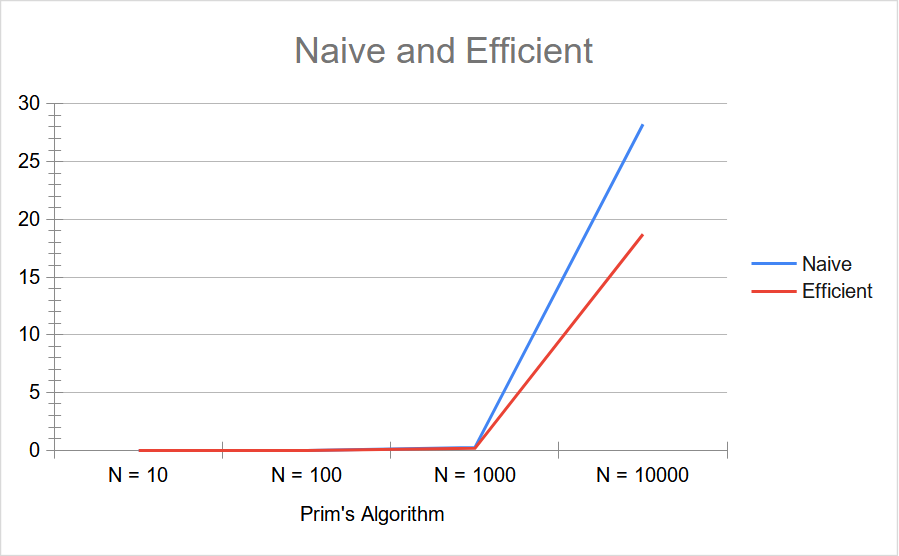
\includegraphics[width=0.75\textwidth]{Prim.png}\par\vspace{1cm}
\end{center}
\begin{center}
  \centering
\end{center}
\subsection{Kruskal's Algorithm}
\begin{center}
  \centering
    \begin{tabular}{|c|c|c|c|c|c|}
    \hline
    \textbf {Algorithm} & \textbf {Time Complexity} & \textbf {N = 10} & \textbf {N = 100} & \textbf {N = 1000} & \textbf {N = 10000}\\
    \hline
    Naive & O($E^2+E.log(V)$) & $0.000181 $ & $0.005331$ & $0.289580 $ & $35.557142$\\
    \hline 
    Efficient & O($E.log(E)+E.log(V)$) & $0.000122 $ & $0.004589  $ & $0.479486  $ & $26.814976$  \\
    \hline
  \end{tabular}
        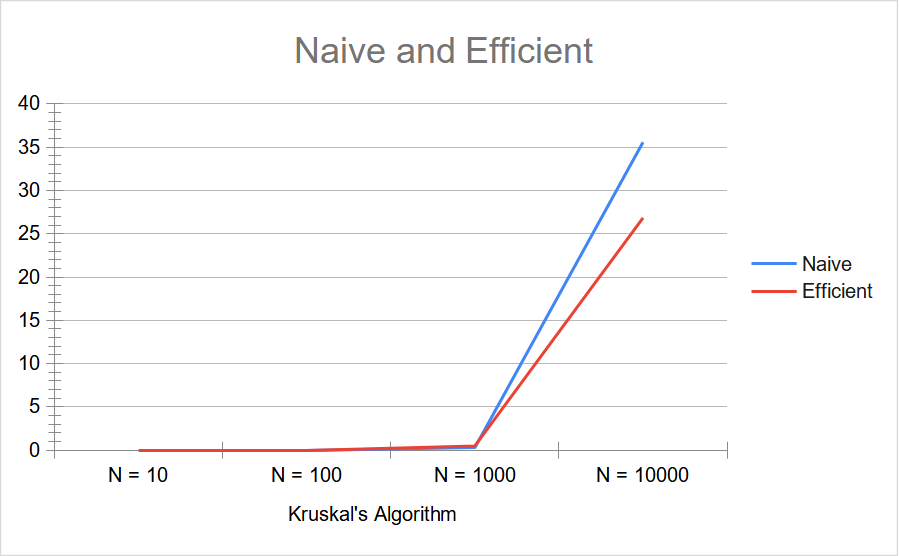
\includegraphics[width=0.75\textwidth]{Kruskal.png}\par\vspace{1cm}
\end{center}
\begin{center}
  \centering
\end{center}
\twocolumn
The above tables show the execution times of each algorithm on graphs with a different number of nodes.
\begin{itemize}
    \item The efficient versions of Prim’s and Kruskal’s algorithms are faster than the naive versions as the size of the graphs becomes large, as expected from their time complexities.
    \item The execution time of the algorithms increases with the size as more vertices and edges require more computations.
    \item The execution time of Prim’s algorithm is more sensitive to the density of the graph than the size, as the algorithm depends on the number of edges that connect the MST to the rest of the graph. The execution time of Kruskal’s algorithm is more sensitive to the size of the graph than the density, as the algorithm depends on the number of edges that need to be sorted and checked for cycles.
    \item The execution time of Prim’s algorithm is lower than Kruskal’s algorithm on dense graphs, as the algorithm adds fewer edges to the MST and avoids unnecessary comparisons. The execution time of Kruskal’s algorithm is lower than Prim’s algorithm on sparse graphs, as the algorithm sorts the edges only once and uses the union-find data structure to efficiently check for cycles.
\end{itemize}

\section{Conclusion}
% Your conclusion content here
In this project, we implemented and compared the naive and efficient versions of Prim’s and Kruskal’s algorithms for finding a minimum spanning tree of a graph using Python. We tested the performance of the algorithms on different types of graphs and analyzed the results. 

Our findings revealed that the efficient versions of the algorithms are faster than the naive versions for large datasets, and that the execution time of the algorithms depends on the size and density of the graphs. Furthermore, we discovered that Prim’s algorithm is more suitable for dense graphs, while Kruskal’s algorithm is more suitable for sparse graphs.

When applied to the optimization of fibre optic trajectory networks, our results indicated that the choice of algorithm can significantly impact the efficiency and cost-effectiveness of the network design. Specifically, for dense networks with numerous potential connection points, Prim’s algorithm provided a more optimal solution. Conversely, for sparse networks with fewer connection points, Kruskal’s algorithm proved to be more effective. 

These findings provide valuable insights for network engineers and designers in the telecommunications industry, helping them to choose the most appropriate algorithm for their specific network topology and thereby optimize the performance and cost-efficiency of their fibre optic trajectory networks.
\subsection{Unexpected Observations}
One of the unexpected observations that we made during this project was that the efficient version of Prim’s algorithm performed worse than the naive version on some very sparse graphs and small graphs. This is because the heap data structure that we used for the efficient version has a higher overhead than the list data structure that we used for the naive version, and the benefit of using the heap is not significant when the number of edges is very small. This suggests that the choice of data structure for implementing the algorithms is not trivial and may depend on the characteristics of the input graph.
\subsection{Challenges Faced}
One of the challenges that we faced during this project was to ensure the validity and correctness of the MSTs that we obtained from the algorithms. We used several methods to verify the MSTs, such as checking if they are connected, acyclic, and contain all the vertices of the original graph, and comparing their weights with the expected values. We also used the implementation of the two versions of Prims's and Kruskal's algorithms using C++ to generate the MSTs compared them with our results. We found that Python results matched with those of C++, which gave us confidence in our implementations.
\subsection{Potential Areas for Future Research or Improvements}
There are several potential areas for future research or improvements for this project, such as:
    \begin{itemize}
        \item Exploring other algorithms for finding an MST, such as Boruvka’s algorithm, which is another greedy algorithm that works by merging components of the MST in parallel.
        \item Implementing parallel or distributed versions of the algorithms, which can take advantage of multiple processors or machines to speed up the computations and handle larger graphs.
        \item Applying the algorithms to real-world problems or datasets, such as road networks, social networks, or image segmentation, and evaluating their performance and usefulness.
        \item Extending the algorithms to handle graphs with negative edge weights, which may require modifications to avoid cycles or negative cycles.
    \end{itemize}
\newpage
\onecolumn
\section{References \& Citations}
% Your references content here
\begin{itemize}
    \item \href{https://leptonsoftware.medium.com/optimizing-fiber-network-management-for-maximum-efficiency-444927851a28}{$https://leptonsoftware.medium.com/optimizing-fiber-network-management-for-maximum-efficiency-444927851a28$}
    \item \href{https://www.geeksforgeeks.org/kruskals-algorithm-simple-implementation-for-adjacency-matrix/}{$https://www.geeksforgeeks.org/kruskals-algorithm-simple-implementation-for-adjacency-matrix/$}
    \item \href{https://www.geeksforgeeks.org/prims-minimum-spanning-tree-mst-greedy-algo-5/}{$https://www.geeksforgeeks.org/prims-minimum-spanning-tree-mst-greedy-algo-5/$}
    \item \href{Karin R Saoub - Graph Theory_ An Introduction to Proofs, Algorithms, and Applications (2021, Chapman and Hall_CRC)}{$Karin R Saoub-Graph Theory-An Introduction to Proofs, Algorithms, and Applications (2021, Chapman and Hall-CRC)$}
    \item \href{Rosen, Kenneth H - Discrete mathematics and its applications-McGraw-Hill (2019)}{$Rosen, Kenneth H - Discrete mathematics and its applications-McGraw-Hill (2019)$}
\end{itemize}

\end{document}